<%# some convenience definitions %>
<%# wiki = @wiki %>
<% full = wiki.filter.clone; full.include_all_namespaces %>
<% wiki.filter.namespace=0 %>
<% users = @wiki.users %>
<% pages = @wiki.pages %>
<% revisions = @wiki.revisions %>
<% topdf = (ENV['RB_TOPDF'] || 'pspdf').to_sym %>
\documentclass{scrartcl}

\usepackage[T1]{fontenc}
\usepackage{booktabs}
\usepackage{graphicx}
\usepackage{subfigure}
\usepackage{tabularx}

\title{Mediawiki Report -- <%= wiki.to_s %>
}
\author{mediawikiparser (<\texttt{klaus.stein@uni-bamberg.de}>)}


\begin{document}
\maketitle

\section{Introduction} % (fold)
\label{sec:introduction}

Florian, Florian, Florian, Florian, Florian, Florian, Florian, Florian, Florian, Florian, Florian, Florian, Florian, Florian, Florian, Florian, Florian, Florian, Florian, Florian, Florian, Florian, Florian, Florian, Florian, Florian, Florian, Florian, Florian, Florian, Florian, Florian, Florian, Florian, Florian, Florian, Florian, Florian, Florian, Florian, Florian, Florian, Florian, Florian, Florian, Florian, Florian, Florian, Florian, Florian, Florian, Florian, Florian, Florian, Florian, Florian, Florian, Florian, Florian, Florian, Florian, Florian, Florian, Florian, Florian, Florian, Florian, Florian, Florian, Florian, Florian, Florian, Florian, Florian, Florian, Florian, Florian, Florian, Florian, Florian, Florian, Florian, Florian, Florian, Florian, Florian, Florian, Florian, Florian, Florian, Florian, Florian, Florian, Florian, Florian, Florian, Florian, Florian, Florian, Florian

% section introduction (end)

\section{Statistics} % (fold)
\label{sec:statistics}

We have <%=@wiki.pages(full).length%> pages with 
<%=@wiki.revisions(full).length%>  revisions from <%=users.length%> 
users (<%=pages.length%> pages with <%=revisions.length%> revisions in 
Namespace 0).

Florian, Florian, Florian, Florian, Florian, Florian, Florian, Florian, Florian, Florian, Florian, Florian, Florian, Florian, Florian, Florian, Florian, Florian, Florian, Florian, Florian, Florian, Florian, Florian, Florian, Florian, Florian, Florian, Florian, Florian, Florian, Florian, Florian, Florian, Florian, Florian, Florian, Florian, Florian, Florian, Florian, Florian, Florian, Florian, Florian, Florian, Florian, Florian, Florian, Florian, Florian, Florian, Florian, Florian, Florian, Florian, Florian, Florian, Florian, Florian, Florian, Florian, Florian, Florian, Florian, Florian, Florian, Florian, Florian, Florian, Florian, Florian, Florian, Florian, Florian, Florian, Florian, Florian, Florian, Florian, Florian, Florian, Florian, Florian, Florian, Florian, Florian, Florian, Florian, Florian, Florian, Florian, Florian, Florian, Florian, Florian, Florian, Florian, Florian, Florian

\subsection{Wiki Statistics} % (fold)
\label{sub:wiki_statistics}

\begin{tabular}{>{\bfseries}lrrrrr}\toprule
  &\textbf{avg} &\textbf{stddev} &\textbf{med} &\textbf{min}
  &\textbf{max}\\
\midrule
<%= 
wiki.global_userstats.collect { |a|
  a.collect { |v| 
    if v.kind_of?(String)
      v
    elsif v.integer? 
      '%5i' % v
    elsif v.nan?
      '---'
    else
      '%7.2f' % v
    end
  }.join('&')
}.join('\\\\')
%>      
\\\bottomrule
\end{tabular}

Florian, Florian, Florian, Florian, Florian, Florian, Florian, Florian, Florian, Florian, Florian, Florian, Florian, Florian, Florian, Florian, Florian, Florian, Florian, Florian, Florian, Florian, Florian, Florian, Florian, Florian, Florian, Florian, Florian, Florian, Florian, Florian, Florian, Florian, Florian, Florian, Florian, Florian, Florian, Florian, Florian, Florian, Florian, Florian, Florian, Florian, Florian, Florian, Florian, Florian, Florian, Florian, Florian, Florian, Florian, Florian, Florian, Florian, Florian, Florian, Florian, Florian, Florian, Florian, Florian, Florian, Florian, Florian, Florian, Florian, Florian, Florian, Florian, Florian, Florian, Florian, Florian, Florian, Florian, Florian, Florian, Florian, Florian, Florian, Florian, Florian, Florian, Florian, Florian, Florian, Florian, Florian, Florian, Florian, Florian, Florian, Florian, Florian, Florian, Florian

% subsection wiki_statistics (end)

\subsection{User Statistics} % (fold)
\label{sub:user_statistics}

\begin{tabular}{>{\bfseries}llrrrrr}\toprule
\textbf{User} & & \textbf{\#edits} & \textbf{\#pages} &
\textbf{edits/page} & \textbf{\#self edits} & \textbf{\#foreign
  edits}\\
\midrule
<%= 
wiki.userstats.sort_by { |u,| u.name }.collect { |u,values| 
  ([u.name, u.node_id] + values[0..4].collect { |v|
     if v.kind_of?(String)
       v
     elsif v.integer? 
       '%5i' % v
     elsif v.nan?
       '---'
     else
       '%7.2f' % v
     end
   }).join('&')
}.join('\\\\')
%>
\\\bottomrule
\end{tabular}

Florian, Florian, Florian, Florian, Florian, Florian, Florian, Florian, Florian, Florian, Florian, Florian, Florian, Florian, Florian, Florian, Florian, Florian, Florian, Florian, Florian, Florian, Florian, Florian, Florian, Florian, Florian, Florian, Florian, Florian, Florian, Florian, Florian, Florian, Florian, Florian, Florian, Florian, Florian, Florian, Florian, Florian, Florian, Florian, Florian, Florian, Florian, Florian, Florian, Florian, Florian, Florian, Florian, Florian, Florian, Florian, Florian, Florian, Florian, Florian, Florian, Florian, Florian, Florian, Florian, Florian, Florian, Florian, Florian, Florian, Florian, Florian, Florian, Florian, Florian, Florian, Florian, Florian, Florian, Florian, Florian, Florian, Florian, Florian, Florian, Florian, Florian, Florian, Florian, Florian, Florian, Florian, Florian, Florian, Florian, Florian, Florian, Florian, Florian, Florian

% subsection user_statistics (end)

% section statistics (end)

%%% Cummulative Distribution Functions: Lorenz, Gini, Pareto %%%

\section{Cummulative Distribution Functions} % (fold)
\label{sec:cummulative_distribution_functions}

% Authors vs. Revisions
<%
ur = users.collect { |u| u.revisions.length }
ur.gp_plot_lorenz(:title => "Lorenz Curve", :xlabel => "authors", :ylabel => "revisions", topdf => 'cdfar.pdf')
%>

% Authors vs. Pages
<%
up = users.collect { |u| u.pages.length }
up.gp_plot_lorenz(:title => "Lorenz Curve", :xlabel => "authors", :ylabel => "pages", topdf => 'cdfap.pdf')
%>

% Revisions vs. Pages
<%
pr = pages.collect { |p| p.revisions.length }
pr.gp_plot_lorenz(:title => "Lorenz Curve", :xlabel => "pages", :ylabel => "revisions", topdf => 'cdfpr.pdf')
%>

\begin{figure}[htbp]
	\centering
	\subfigure[Authors vs. Revisions]{\includegraphics[width=0.5\textwidth]{cdfar}}\\
	\subfigure[Authors vs. Pages]{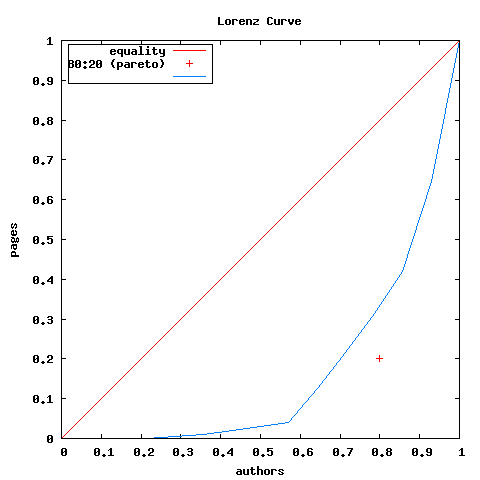
\includegraphics[width=0.5\textwidth]{cdfap}}\\
	\subfigure[Revisions vs. Pages]{\includegraphics[width=0.5\textwidth]{cdfpr}}
	\caption{Cummulative Distribution Functions}
	\label{fig:cummulative_distribution_functions}
\end{figure}

Florian, Florian, Florian, Florian, Florian, Florian, Florian, Florian, Florian, Florian, Florian, Florian, Florian, Florian, Florian, Florian, Florian, Florian, Florian, Florian, Florian, Florian, Florian, Florian, Florian, Florian, Florian, Florian, Florian, Florian, Florian, Florian, Florian, Florian, Florian, Florian, Florian, Florian, Florian, Florian, Florian, Florian, Florian, Florian, Florian, Florian, Florian, Florian, Florian, Florian, Florian, Florian, Florian, Florian, Florian, Florian, Florian, Florian, Florian, Florian, Florian, Florian, Florian, Florian, Florian, Florian, Florian, Florian, Florian, Florian, Florian, Florian, Florian, Florian, Florian, Florian, Florian, Florian, Florian, Florian, Florian, Florian, Florian, Florian, Florian, Florian, Florian, Florian, Florian, Florian, Florian, Florian, Florian, Florian, Florian, Florian, Florian, Florian, Florian, Florian

% section cummulative_distribution_functions (end)

%%% Set Filter and Time Raster %%%
<%
filter = wiki.filter.clone # clone filter
raster = wiki.timeraster(:zero => :week, :step => :week) # set time raster to weekly spells
%>

\section{Revision History} % (fold)
\label{sec:revision_history}

% Revisions per Week (RPW)
<% 
rpw = raster[1..-2].enum_cons(2).collect { |s,e| 
	filter.revision_timespan = (s..e)
	[ e, wiki.revisions(filter).length ]
	}
Gnuplot.new do |gp|
	gp.set('xdata', 'time')
	gp.set('timefmt', '%Y-%m-%d', true)
	gp.set('format x', '%b %y', true)
	gp.add(rpw, :timefmt => '%Y-%m-%d',
		:with => 'lines', 
		:title => 'revisions' )
	gp.set('xtics rotate')
	gp.set('title "Revisions per Week"')
	gp.set('xlabel "month"')
	gp.set('ylabel "number of revisions"')
	gp.fit(:title => 'trend')
	gp.plot(:svg => 'rpw.svg')
	gp.plot(topdf => 'rpw.pdf')
end
%>
\begin{figure}[htbp]
	\centering
	\includegraphics[width=0.95\textwidth]{rpw}
	\caption{Revisions per Week}
	\label{fig:revisions_per_week}
\end{figure}

Florian, Florian, Florian, Florian, Florian, Florian, Florian, Florian, Florian, Florian, Florian, Florian, Florian, Florian, Florian, Florian, Florian, Florian, Florian, Florian, Florian, Florian, Florian, Florian, Florian, Florian, Florian, Florian, Florian, Florian, Florian, Florian, Florian, Florian, Florian, Florian, Florian, Florian, Florian, Florian, Florian, Florian, Florian, Florian, Florian, Florian, Florian, Florian, Florian, Florian, Florian, Florian, Florian, Florian, Florian, Florian, Florian, Florian, Florian, Florian, Florian, Florian, Florian, Florian, Florian, Florian, Florian, Florian, Florian, Florian, Florian, Florian, Florian, Florian, Florian, Florian, Florian, Florian, Florian, Florian, Florian, Florian, Florian, Florian, Florian, Florian, Florian, Florian, Florian, Florian, Florian, Florian, Florian, Florian, Florian, Florian, Florian, Florian, Florian, Florian

%%% Set Filter and Time Raster %%%
<%
filter = wiki.filter.clone # clone filter
raster = wiki.timeraster(:zero => :week, :step => :week) # set time raster to weekly spells
%>

% Cummulative Revisions per Week (CRPW)
<% 
crpw = raster[1..-2].collect { |e| filter.endtime = e 
	[ e, wiki.revisions(filter).length ]
	}
Gnuplot.new do |gp|
	gp.set('xdata', 'time')
	gp.set('timefmt', '%Y-%m-%d', true)
	gp.set('format x', '%b %y', true)
	gp.add(crpw, :timefmt => '%Y-%m-%d', 
		:with => 'linespoints', 
		:title => 'revisions')
	gp.set('nokey')
	gp.set('xtics rotate')
	gp.set('title "Cummulative Revisions per Week"')
	gp.set('xlabel "month"')
	gp.set('ylabel "cummulative number of revisions"')
	gp.plot(topdf => 'crpw.pdf')
end
%>
\begin{figure}[htbp]
	\centering
	\includegraphics[width=0.95\textwidth]{crpw}
	\caption{Cummulative Revisions per Week}
	\label{fig:cummulative_revisions_per_week}
\end{figure}

Florian, Florian, Florian, Florian, Florian, Florian, Florian, Florian, Florian, Florian, Florian, Florian, Florian, Florian, Florian, Florian, Florian, Florian, Florian, Florian, Florian, Florian, Florian, Florian, Florian, Florian, Florian, Florian, Florian, Florian, Florian, Florian, Florian, Florian, Florian, Florian, Florian, Florian, Florian, Florian, Florian, Florian, Florian, Florian, Florian, Florian, Florian, Florian, Florian, Florian, Florian, Florian, Florian, Florian, Florian, Florian, Florian, Florian, Florian, Florian, Florian, Florian, Florian, Florian, Florian, Florian, Florian, Florian, Florian, Florian, Florian, Florian, Florian, Florian, Florian, Florian, Florian, Florian, Florian, Florian, Florian, Florian, Florian, Florian, Florian, Florian, Florian, Florian, Florian, Florian, Florian, Florian, Florian, Florian, Florian, Florian, Florian, Florian, Florian, Florian

% section revision_history (end)

\section{Author Participation} % (fold)
\label{sec:author_participation}

%%% Set Filter and Time Raster %%%
<%
filter = wiki.filter.clone # clone filter
raster = wiki.timeraster(:zero => :week, :step => :week) # set time raster to weekly spells
%>

% Author Participation per Week
<%
# authors
authors = raster.enum_cons(2).collect { |s,e| 
	filter.revision_timespan = (s..e)
	[ e, wiki.coauthorgraph(filter).remove_lonely_nodes.nodes.length ]
}[1..-2]
# Gnuplot
Gnuplot.new do |gp|
	gp.set('xdata', 'time')
	gp.set('timefmt', '%Y-%m-%d', true)
	gp.set('format x', '%b %y', true)
	gp.add(authors, :timefmt => '%Y-%m-%d',
		:with => 'lines',
		:title => 'authors')
	gp.set('nokey')
	gp.set('xtics rotate')
	gp.set('title "Author Participation"')
	gp.set('xlabel "month"')
	gp.set('ylabel "number of authors"')
	gp.fit(:title => 'trend')
	gp.plot(topdf => 'author_participation.pdf')
end
%>
\begin{figure}[htbp]
	\centering
	\includegraphics[width=0.95\textwidth]{author_participation}
	\caption{Author Participation}
	\label{fig:author_participation}
\end{figure}

Figure~\ref{fig:author_participation} shows the number of authors who edited at least one document at any given week. While the absolute numbers are likely to fluctuate, the trend line gives an idea of just how many authors participate in the wiki.

% Relative Author Participation per Week
<%
# events
events = wiki.users.collect{ |u| 
	[ u.time_of_first_event, u.time_of_last_event ] 
    }.select { |f,l| f && l }
# authors
authors = raster.enum_cons(2).collect { |s,e|
	filter.revision_timespan = (s..e)
	[ e,
    	wiki.coauthorgraph(filter).remove_lonely_nodes.nodes.length /
        events.reject { |f,l| (f > e) || (l < s) }.length.to_f ]
	}[1..-2]
# Gnuplot
Gnuplot.new do |gp|
	gp.set('xdata', 'time')
	gp.set('timefmt', '%Y-%m-%d', true)
	gp.set('format x', '%b %y', true)
	gp.add(authors, :timefmt => '%Y-%m-%d',
		:with => 'lines',
		:title => 'authors')
	gp.set('nokey')
	gp.set('xtics rotate')
	gp.set('title "Relative Author Participation"')
	gp.set('xlabel "month"')
	gp.set('ylabel "percentage of authors"')
	gp.fit(:title => 'trend')
	gp.plot(topdf => 'relative_author_participation.pdf', :size => '640,480')
end
%>

\begin{figure}[htbp]
	\centering
	\includegraphics[width=0.95\textwidth]{relative_author_participation}
	\caption{Relative Author Participation}
	\label{fig:relative_author_participation}
\end{figure}

Figure~\ref{fig:relative_author_participation} shows the percentage of authors who edit at least one document at any given week. For example, a value of 50\,\% indicates that half of all active authors participate in the wiki. Note that we define an author as active for the time between his first and his last edit. Therefore, and in contrast to Figure~\ref{fig:author_participation}, relative author participation adjusts for growth of the wiki in question. Again, while the absolute percentages are likely to fluctuate, the trend line gives an idea of just the percentage of authors who participate in the wiki.

% section author_participation (end)

\section{Network Visualization} % (fold)
\label{sec:network_visualization}

% Co-Authorship Network
<%
filter = wiki.filter.clone # clone filter
coauthorship_network = wiki.coauthorgraph(filter) { |n| [ "label=\"\"" ] }.remove_self_links.remove_lonely_nodes
coauthorship_network.to_graphviz("coauthorgraph.pdf", "neato", :pdf, "outputorder=edgesfirst", "node [ shape=point, style=filled, fillcolor=white ]" ) { |w|  "[ weight=#{w} ]" }
%>
\begin{figure}[htbp]
	\centering
	\includegraphics[width=0.95\textwidth]{coauthorgraph}
	\caption{Coauthorship Network}
	\label{fig:coauthorship_network}
\end{figure}

Figure~\ref{fig:coauthorship_network} shows the coauthorship network in which the nodes are authors, and a link between any two nodes represents authorship of one or more pages. There are <%= coauthorship_network.nodes.length %> nodes connected by <%= coauthorship_network.links.length %> links in the network. The coauthorship network gives an idea of who is working with whom. Single nodes with above average links to others identify authors who work with many others, usually on many pages. Rather than content, these authors provide most of the structure to the wiki. Clusters of nodes identify authors working in close concert with each other. These authors provide most of the content to the wiki.


%%% TO DO %%%
% Top 5 Authors in terms of Revisions, Degree, Betweenness, Closeness
% wiki.coauthorgraph.nodes.sort_by { |n| -n.revisions.length }.collect { |n| [ n.name, n.revisions.length ] }[0..4]
% wiki.coauthorgraph.degrees.collect { |k,v| [ k, v[0] + v[1] ] }.sort_by { |k,v| -v }.collect { |k,v| [ k.name, v ] }[0..4]
% wiki.coauthorgraph.betweenness.sort_by { |k,v| -v }.collect { |k,v| [ k.name, v ] }[0..4]
% wiki.coauthorgraph.closeness.sort_by { |k,v| -v }.collect { |k,v| [ k.name, v ] }[0..4]
%%% TO DO %%%

% Document Network
<%
filter = wiki.filter.clone # clone filter
page_network = wiki.pagegraph(filter) { |n| [ "label=\"\"" ] }.remove_self_links.remove_lonely_nodes
page_network.to_graphviz("pagegraph.pdf", "neato", :pdf, "outputorder=edgesfirst", "node [ shape=point, style=filled, fillcolor=white ]" ) { |w|  "[ weight=#{w} ]" }
%>

\begin{figure}[htbp]
	\centering
	\includegraphics[width=0.95\textwidth]{pagegraph}
	\caption{Page Network}
	\label{fig:page_network}
\end{figure}

Figure~\ref{fig:page_network} shows the page network in which the nodes are pages, and a link between any two nodes represents a hyperlink from one to the other page. There are <%= page_network.nodes.length %> nodes connected by <%= page_network.links.length %> links in the network.  The page network gives an idea of which page links to which other. Single nodes with above average links to others identify pages which serve as portals. These pages provide most of the structure of the wiki. Clusters of nodes identify pages which revolve around a common theme or topic. These pages provide most of the content of the wiki.


%%% TO DO %%%
% Top 10 Pages (Indegree)
% wiki.pagegraph.degrees.collect {|k,v| [ k, v[0] ] }.sort_by { |k,v| -v }.collect { |k,v| [ k.title, k.revisions.length, v ] }[0..9]
%\begin{tabular}{>{\bfseries}llrrrrr}
%	\toprule
%	\textbf{Title} & \textbf{Indegree} & \textbf{Revisions} &
%...

% Top 10 Pages (Outdegree)
% wiki.pagegraph.degrees.collect {|k,v| [ k, v[1] ] }.sort_by { |k,v| -v }.collect { |k,v| [ k.title, k.revisions.length, v ] }[0..9]
%\begin{tabular}{>{\bfseries}llrrrrr}
%	\toprule
%	\textbf{Title} & \textbf{Outdegree} & \textbf{Revisions} &
%...
%%% TO DO %%%

% section network_visualization (end)

\end{document}
